\chapter{Arkitektur}
Dette afsnit vil forsøge at beskrive de valg der blevet foretaget ifht. arkitekturen bag BargainBarter. Der vil kort blive beskrevet om de enkelte begreber og arkitekturstile der blev anvendt til at opbygge systemet og en begrundelse af disse valg.

\section{Arkitektur stile}
Da der i projektet ønskes at udvikle en webapplikation, så er det derfor nødvendigt at anvende en arkitekturstil, der fungerer til dette formål. 
Dette valg faldt på 3-lags modellen, da denne model anvendes meget i forbindelse med udvikling af hjemmesider. 3-lags modellen består af:
\begin{enumerate}
	\item En front-end web-server der leverer statisk eller dynamisk materiale - dvs. al det materiale der vises i webbrowseren.
	\item Et lag der generer og processere dynamisk materiale.
	\item En back-end database til at gemme og hente data fra.
\end{enumerate}

Modellen sørger for lav kobling mellem de forskellige dele/lag. Denne model består af et Presentation Layer, Business Logic Layer og et Data Access Layer. Denne model gør det muligt at skifte de forskellige lag ud, hvis det skulle vise sig at være nødvendigt. Det betyder desuden også at det er nemmere at teste de forskellige dele af systemet. \\
For yderligere information henvises der til dokumentation. \footnote{Se bilag - Dokumentation, sektion xx}

\section{Teknologivalg}
I denne sektion vil de specifikke teknologier, der er anvendt i projektet, blive beskrevet.

\subsection{ASP.NET MVC}
Frameworket ASP.NET MVC\cite{MVC} fra Microsoft blev valgt som platform til webapplikationen, da dette framework har utallige fordele i forhold til dette projekt. 
\begin{enumerate}
	\item ASP.NET MVC understøtter .NET frameworket, hvilket muliggøre  udvikling i C\#.
	\item Frameworket har eksisteret i mange år og er derfor veldokumenteret og mange biblioteker understøtter dette framework.
	\item Gruppen har modtaget undervisning i ASP.NET MVC.
\end{enumerate}
Der er en masse andre framework, der kunne have været interessante at anvende, såsom Ruby on Rails, men disse framework anvender ikke .NET eller C\#, hvilket gruppen var vigtigt, at frameworket understøttede.

\noindent På figur \ref{fig:MVC} kan der ses den overordnet struktur af den 3-lags model ASP.NET MVC er bygget på. \\
Model er den del der arbejder med den data relaterede logik, dvs. Data Acces Layer. Det er altså al den data der tages fra databasen og bliver manipuleret af Views eller Controllers.\\
View er præsentations logikken. \\
Controller er bindeleddet mellem Model og Views. Dens opgaave er at manipulere data fra modellen og interagere med Views for at vise outputtet og modtage inputs fra viewet. \\ 

\begin{figure}[H]
	\centering
	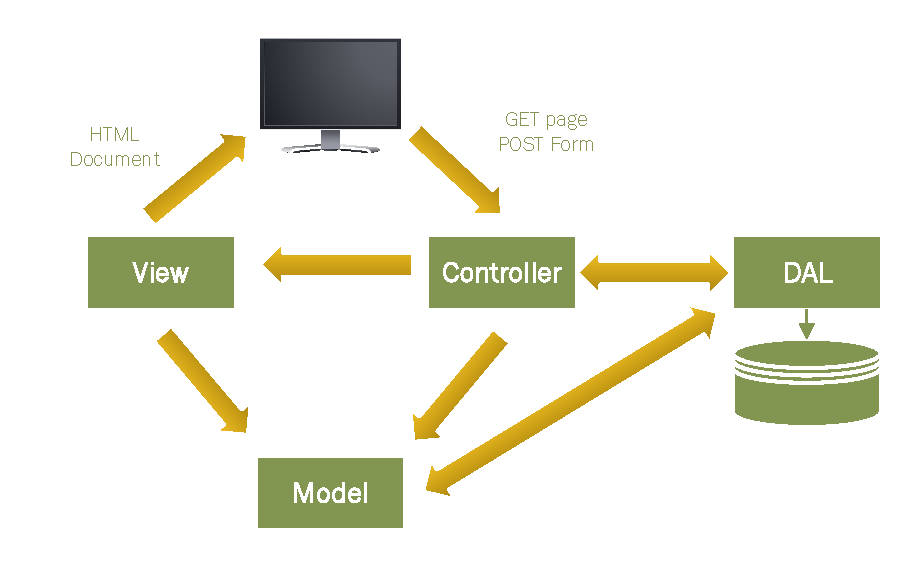
\includegraphics
	[width=140mm]{figures/MVC_drawing.pdf}
	\caption{MVC struktur}
	\label{fig:MVC}
\end{figure}

\subsection{Data Access Layer}
I forbindelse med database adgangen blev Entity Framework anvendt.
 
 \subsubsection{Entity Framework}
Entity framework (EF)\cite{ADOEF} var det oplagte valg, når først ASP.NET MVC var valgt. EF kommer som standard når der oprettes et ASP.NET MVC projekt, og opretter selv en skabelon til at oprette database tabeller. EF er et object-relational mapping (ORM) framework til ADO.NET, der understøtter udviklingen af data orienterede applikationer. Det vil sige, at EF sørger for en bekvemmelig og ensartet tilgang til den database man anvender til at gemme og hente data til viewet. \\
 \noindent Til selve databasen er der anvendt SQL Server 2016, som IHA har stillet til rådighed.
 
\subsection{Presentation Layer}
Til præsentations laget anvendes der HTML/CSS til at præsentere data for brugeren. Da brugervenlighed var centralt for systemet blev Bootstrap\cite{Bootstrap} anvendt. Bootstrap er et framework, der gør webapplikationen responsive og skalebare. Frameworket gør det nemt at designe et View der kan skaleres til en hvilken som helst skærm - uanset om det er mobil, tablet eller desktop. Desuden indeholder Bootstrap en række temaer, der gør det enkelt at designe et View der er pænt, hvilket ikke gruppens stærke side. \\
For at gøre View'et mere dynamisk er der anvendt Javascript og mere specifikt JQuery\cite{jQuery}. 
Dette bibliotek gør det muligt f.eks. at vise popup vinduer, hvis der er brug for det eller i gruppens tilfælde at kunne bedømme en anden bruger.